\pagestyle{fancy}

\graphicspath{ {Figures/Chapter1_Overview/} }

\section{CERN accelerators complex}
\label{sec:CERN_acc_complex}

The European Organization for Nuclear Research (CERN) was founded in 1954, and it has become the largest particle physics laboratory in the world \parencite*[][]{ref:CernWebsite}. It sits astride the FrancoSwiss border near Geneva. It was one of Europe's first joint ventures and now has 23 member states. At CERN, the world's largest and most complex scientific instruments are used to study the basic constituents of matter. However, the physics program at the laboratory is much broader, ranging from nuclear to high-energy physics, from studies of antimatter to the possible effects of cosmic rays on clouds \parencite[][]{ref:PhysProgramCern}. CERN has also pushed the frontiers of technology with inventions such as the Worl Wide Web (www), Proton Emission Tomography (PET), etc.  

\begin{figure}[h]
    \centering
    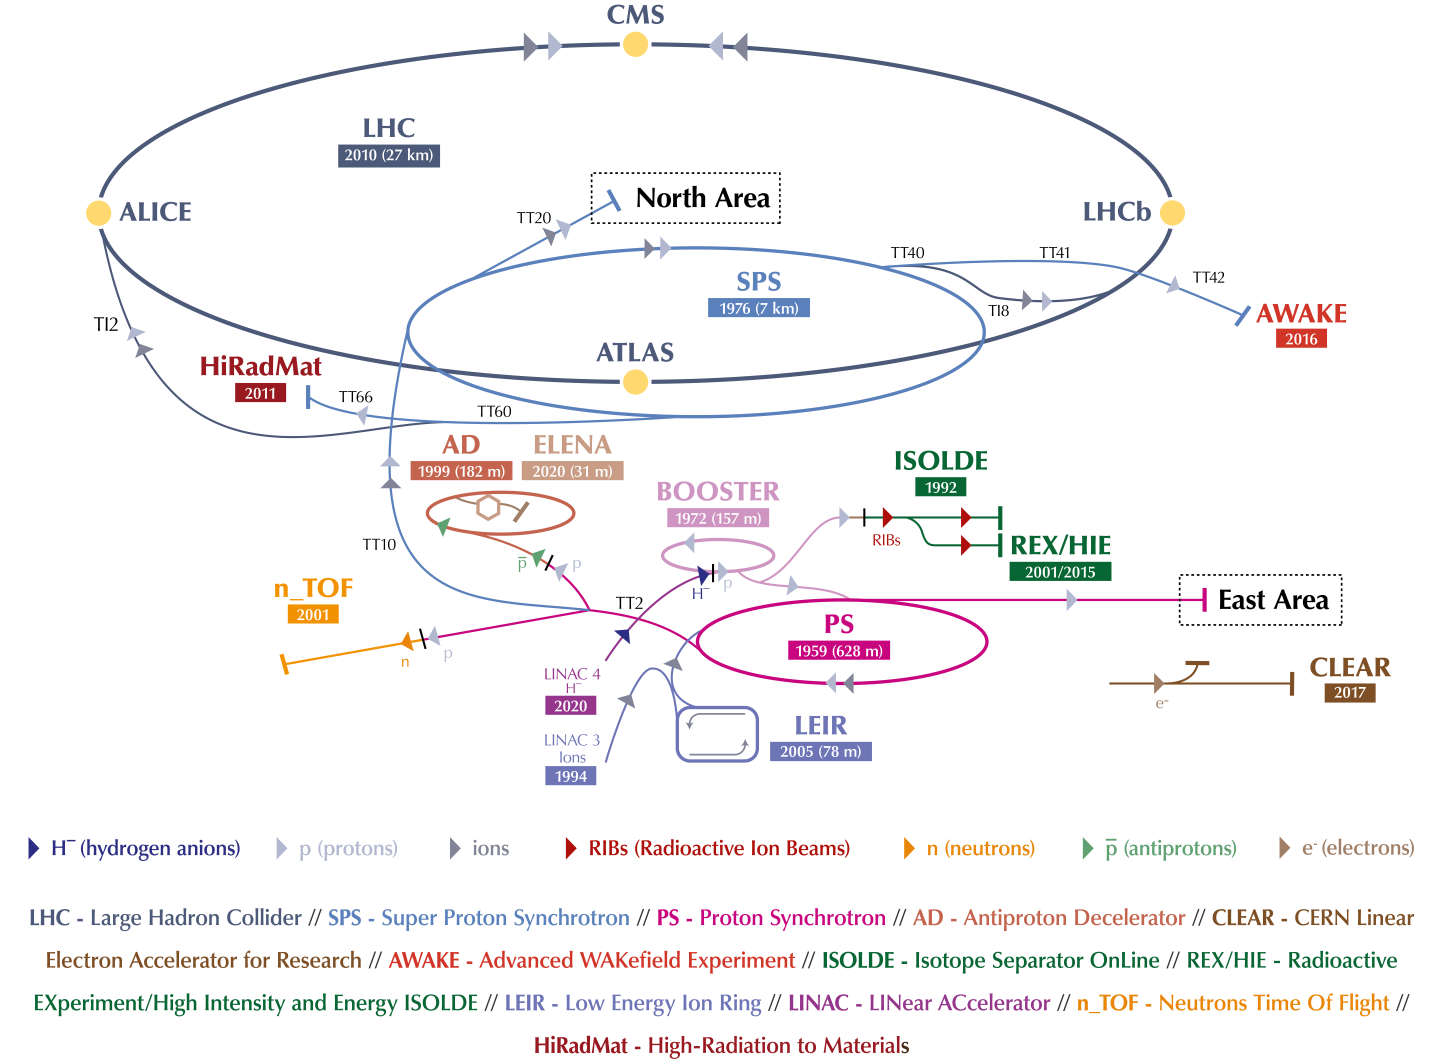
\includegraphics[width=0.9\columnwidth]{Figure_AcceleratorChain/cernComplex.png}
    \caption{CERN Accelerator Complex \parencite*[][]{ref:cerncomplex} . }
    \label{fig:AccComplex}
\end{figure}

CERN's accelerator complex (See \ref{fig:AccComplex} ) consists of many different types of linear and circular accelerators and interconnecting transfer lines to gradually accelerate the particles before injection into the Large Hadron Collider (LHC). 

Since 2020, Linear accelerator 4 (Linac4) became the source of proton beams for the LHC. Linac4 is an 86 \si{\meter} long machine. It accelerates negative hydrogen ions up to 160 \si{\mega \electronvolt}. The ions are then stripped of their two electrons during injection from Linac4 into the Proton Synchrotron Booster (PS Booster or PSB) to leave only protons. The PS Booster is made up of four superimposed synchrotron rings, with a 157 \si{\meter} circumference, which accelerates the injected protons up to 2 GeV for injection into the Proton Synchrotron (PS). 

Currently, the PS is the oldest accelerator in the chain. With a circumference of 628 meters, the PS operates up to 26 \si{\giga \electronvolt}. The Super Proton Synchrotron (SPS) is the second largest machine in the complex, measuring nearly 7 \si{\kilo \meter} in circumference. It takes the particles from the Proton Synchrotron and accelerates them up to 450 \si{\giga \electronvolt}. The CERN accelerator complex culminates with the Large Hadron Collider. The LHC consists of a 27 \si{\kilo \meter} ring of superconducting magnets, which guide two high-energy particle beams traveling in opposite directions in separate beam pipes. The beams collide at four locations around the accelerator ring, corresponding to the positions of four particle detectors ATLAS, CMS, ALICE and LHCb. The High Luminosity Large Hadron Collider ( HiLumi LHC) project aims to deliver proton-proton collisions at 14 \si{\tera \electronvolt}.

Not only protons can be accelerated at the CERN accelerator complex. Linear accelerator 3 (Linac 3) is the starting point for the ions. It usually provides lead ions, but also argon and xenon were used in the past. Experiments with oxygen are planned for the future. The long pulses of lead ions from Linac 3 are transformed into short, dense bunches by the Low Energy Ion Ring (LEIR) before they are injected into the PS. 

The injector chain, apart from feeding the LHC, is also used to deliver particles to several other experiments carried out at CERN, including Antimatter research on the Antiproton Decelerator (AD) and Extra Low ENergy Antiproton (ELENA), radioactive ion beam research on ISOLDE, research on neutron-nucleus interactions on the n-TOF facility, research on radiation-induced damage on materials in the HiRadMat facility and even studies on the use of proton-driven plasma wake-fields in AWAKE. 

\subsection{Linear Accelerator 4 (LINAC4)}
\label{sec:LINAC4}

As part of the LHC injection upgrade (LIU), LINAC4 was introduced to substitute LINAC2  \parencite*[]{ref:LIU}. The main goal for the construction of LINAC4 was to increase the beam brightness. This increase is achieved by combining two effects. Firstly, the increase of the top energy to \SIlist[]{60}{\mega \electronvolt} (compared to the \SI[]{50}{\mega \electronvolt} given by LINAC2), which reduces significantly the space charge effect causing emittance-blow up in the PSB. Secondly, the use of $H^{-}$ ions instead of protons makes it possible to inject into the PSB via the charge exchange injection scheme (explained in detail in Chapter \ref{ch:H0Hm}). During the long shutdown (2019-2020), LINAC4 finally replaced LINAC2 as the source of protons for the LHC. 

Figure \ref{fig:Linac4_acc} shows a description of the accelerating sequence of LINAC4. This sequence is quite standard for a pulsed LINAC design. The LINAC4 source is a cesiated molybdenum-surface radio-frequency plasma ion source \parencite*[][]{ref:SourceCite}. This source can produce $H^{-}$ ion beams of up to 400 \si[]{\micro \second} pulse length, 40 \si[]{\milli \ampere} at a maximum revolution frequency of \SI[]{0.8}{\hertz}

\begin{figure}[h]
    \centering
    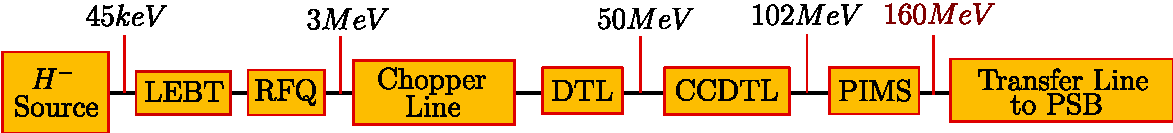
\includegraphics[width=1.0\columnwidth]{Linac4_AcceleratingPart/Linac4_acc.pdf}
    \caption{LINAC4 accelerating components layout. }
    \label{fig:Linac4_acc}
\end{figure}

The Low Energy Beam Transport (LEBT) line provides the beam matching from the source to the RFQ (Radio Frequency Quadrupoles) and contains the diagnostics to monitor the source. The three-meter RFQ performs the beam capture and bunching and accelerates the particles to an energy of 3\si[]{\mega \electronvolt}. It is followed by a Medium Energy Beam Transport (MEBT) or "Chopper Line". This system consists of an electrostatic beam deflector followed by a beam dump. The purpose of this line is to avoid losses at higher energies when the induced radiation is higher.


Three types of losses are treated with this system. Firstly, losses due to instable LINAC4 pulses. Secondly, it can be used to clean the first few tens of \si[]{\micro \second} of the beam pulse which is generally not stable. Finally, its purpose is to create "holes" in the beam pulse, timed with the rise-time of the PSB distributor, which switches the incoming LINAC4 beam between the four PSB Rings.  

\begin{figure}[h]
    \centering
    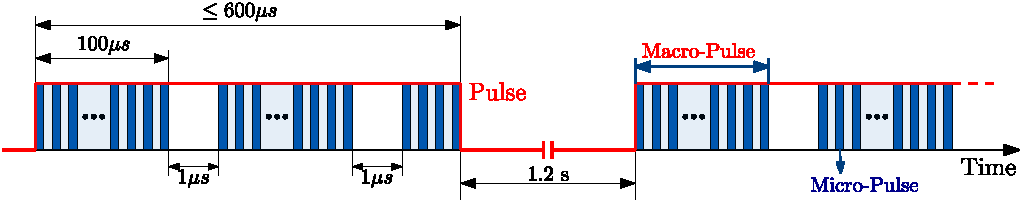
\includegraphics[width=1.0\columnwidth]{Figure_Linac4PulseStructure/Linac4_PulseStruct.pdf}
    \caption{LINAC4 Pulse Structure }
    \label{fig:Linac4PulseStruct}
\end{figure}

The chopping line is followed by a series of three accelerating structures. The Drift Tube Linac (DTL) is divided into three tanks and accelerates the beam up to 50 \si[]{\mega \electronvolt}. The Cell-Coupled Drift Tube Linac (CCDTL) is made of 7 accelerating modules for top energy of 102 \si[]{\mega \electronvolt}. Finally, the Pi-Mode Structure (PIMS) brings the energy of the beam to the desired 160 \si[]{\mega\electronvolt}. More information about LINAC4 and its conforming parts can be found in \parencite*[]{ref:Linac4Technical}.  

In the current operational conditions, the LINAC4 pulse structure consists of four individual macro pulses, typically 20 - 100 \si[]{\micro \second} long (depending on the required number of injected turns per ring) and separated by a 1 \si[]{\micro \second} particle-free gap (See figure \ref{fig:Linac4PulseStruct}). Each macro-pulse consists of a train of 500 \si[]{\pico \second} long micro-bunches that are spaced by intervals of 2.8 \si[]{\nano \second} \parencite*[]{ref:Linac4PulseStruct}.

\newpage

\section{Accelerator Physics Principles}
\label{sec:AccPhysPrinc}

The topic of Accelerator physics is very broad, in this section only an overview of the topics of interest for this document will be introduced. These topics include a quick overview of the basic concepts of beam dynamics, transverse plane, beam size and emittance. For a much more complete introduction to the world of accelerators check \parencite*[][]{ref:BookAccPhysics}.

\subsection{Principles of beam dynamics}
\label{subsec:PrincBeamDyn}

To describe the movement of the particles in an accelerator, the Frenet-Serret coordinate system, shown in figure \ref{fig:CoordinateSystem}, is commonly used. S defines the longitudinal coordinate and it is always tangent to the reference path. X and Y define the transverse plane (orthogonal to the particle trajectory). x(s) and y(s) describe the particle's deviation from the reference path and $\rho(s)$ commonly defines the curvature of the reference orbit at each point. 


\begin{figure}[h]
    \centering
    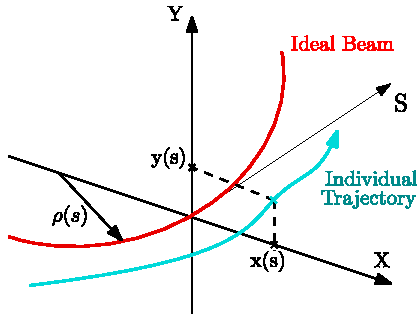
\includegraphics[width=0.5\columnwidth]{Figure_CoordinateSystem/CoordinateSystem.pdf}
    \caption{Frenet-Serret coordinate system.}
    \label{fig:CoordinateSystem}
\end{figure}

The scope of a particle accelerator design is to guide the beam of particles along the reference path and accelerate them to the desired energy. In the simplest case, we consider constant energy and stable beam trajectory. One can guide these particles by applying electromagnetic forces to them. Lorentz's law describes the force acting on a particle of charge "q" traveling in an electromagnetic field:

\begin{equation}
    \vec{F} = q \left( \vec{E} + \vec{v} \times  \vec{B}\right)
    \label{eq:LorentzLaw}
\end{equation}

Where $\vec{E}$ and $\vec{B}$ are the electric and magnetic fields and $\vec{v}$ is the particle velocity. Longitudinal electric fields accelerate the particles, while transverse bending and focusing are provided by transverse magnetic fields. 

Particles which at the time $t_0$ have a non zero transverse coordinate $\left(x_0 , y_0 \right)$ and momentum $\left(x_{0}^{'} , y_{0}^{'} \right)$ start to perform oscillations in the horizontal and vertical planes,  called Betatron oscillations \parencite*[][]{ref:BookAccPhysics2}. These oscillations depend on the magnetic fields in the ring. The equation of motion on the transverse space can be derived from Lorentz's equation, and after some approximations, they read \parencite*[][]{ref:ApproxEqMotion}:

\begin{equation}
    \begin{aligned}
        x^{''} + \left(\frac{1}{\rho^{2}(s)}+\frac{1}{B\rho}\frac{\partial B_y(s)}{\partial x} \right)  x = 0 \\
        y^{''} - \frac{1}{B \rho}\frac{\partial B_y (s)}{\partial x}  y = 0
    \end{aligned}
    \label{eq:EqMotion}
\end{equation}

The product $B \rho$ is the magnetic rigidity and is equal to the ratio of the momentum to charge $p/q$. The only difference between the vertical and horizontal coordinates is the term $1/\rho^2(s)$ which is related to the centripetal force in the radial direction. These types of differential equations are often referred to as Hills equation \parencite*[][]{ref:HillEquation}, and describe a pseudo harmonic oscillator in which the spring constant depends on the position (s). For each element on the beamline, one can calculate the solution of the equation of motion. This solution can be expressed in a matrix formulation \parencite*[][]{ref:MatrixForm}:

\begin{equation}
    \begin{bmatrix}
        u(s) \\ u^{'}(s) 
   \end{bmatrix}
   = 
   \begin{bmatrix}
        C(s) & S(s) \\ C^{'}(s)  & S^{'}(s)
   \end{bmatrix}
   \begin{bmatrix}
        u_0 \\ u^{'}_0
   \end{bmatrix}
   =
   M(s) 
   \begin{bmatrix}
        u_0 \\ u^{'}_0
   \end{bmatrix}
\end{equation}

Where $M(s)$ is called the transformation matrix, which can be calculated individually for each type of beamline element. This matrix formalism is very useful as one can follow a particle trajectory along a complicated beam line by repeated matrix multiplication from element to element \parencite*[][]{ref:MatrixTransport}.

\subsection{Particle beams and beam profile}
\label{subsec:TransBeamProf}

A beam or a bunch of particles is a collection of a very large number of particles whose center of gravity moves in a well-defined direction. If we consider the transverse plane X-Y (orthogonal to the beam direction of motion), one can obtain the particle distribution by noting the position of each particle that crosses this plane. If there is no coupling between the motion of the particles in the x and y directions, the distribution of the particles will be somehow elliptical, with the axis of the ellipse parallel to the x and y axes. See Figure \ref{fig:TransversePlane} for an example of transverse space particle distribution. 

A histogram expressing the number of particles in a beam as a function of the transverse position is known as a beam profile. A Horizontal beam profile gives information about the number of particles at different x positions. A Vertical beam profile gives information about the number of particles at different y positions. A typical way of expressing the number of particles at a certain point in space is using a gaussian function:

\begin{equation}
    N(x,y) = \frac{N_{Tot}}{2\pi\sigma_x \sigma_y}\cdot exp\left(-\frac{1}{2}\left(\left(\frac{x-x_0}{\sigma_x}\right)^2 -\left(\frac{y-y_0}{\sigma_y}\right)^2\right)\right)
    \label{eq:GaussianDist}
\end{equation}

Here $x_0 , y_0$ are the coordinates of the center of the beam. $\sigma_x , \sigma_y$ are the standard deviation of the normally distributed beam of particles. $N_{Tot}$ refers to the total number of particles in the beam pulse. However, this expression is no more than an approximation, and one should be careful to understand its limitations. Usually, at the particle source, the beam of particles is far from Gaussian, but after some acceleration, this becomes a good approximation \parencite*[][]{ref:BookAccPhysics}.

\begin{figure}[t]
    \centering
    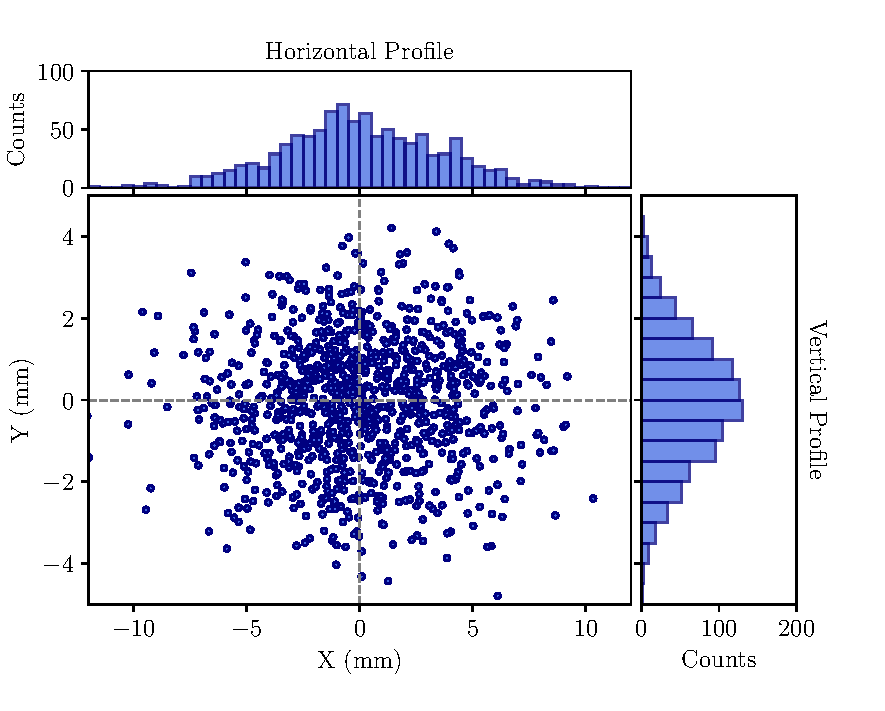
\includegraphics[width=0.9\columnwidth]{Figure_ParticlePositionExample/ParticlePosition.pdf}
    \caption{Example of Particle distribution in the X-Y space, with their corresponding projections.}
    \label{fig:TransversePlane}
\end{figure}

\subsection{Transverse phase space}
\label{subsec:TransPhSp}

Each one of the particles in the beam will not only have a different position, but also a different direction of movement. The velocity vector of each particle can be decomposed into two components, one parallel to the beam direction (s) and one orthogonal to it (transverse velocity). The transverse velocity can then be discomposed into its components along the x-axis and y-axis. The phase space has information on both the position and the transverse velocity of each of the particles in the beam. 

\begin{figure}[h!]
    \centering
    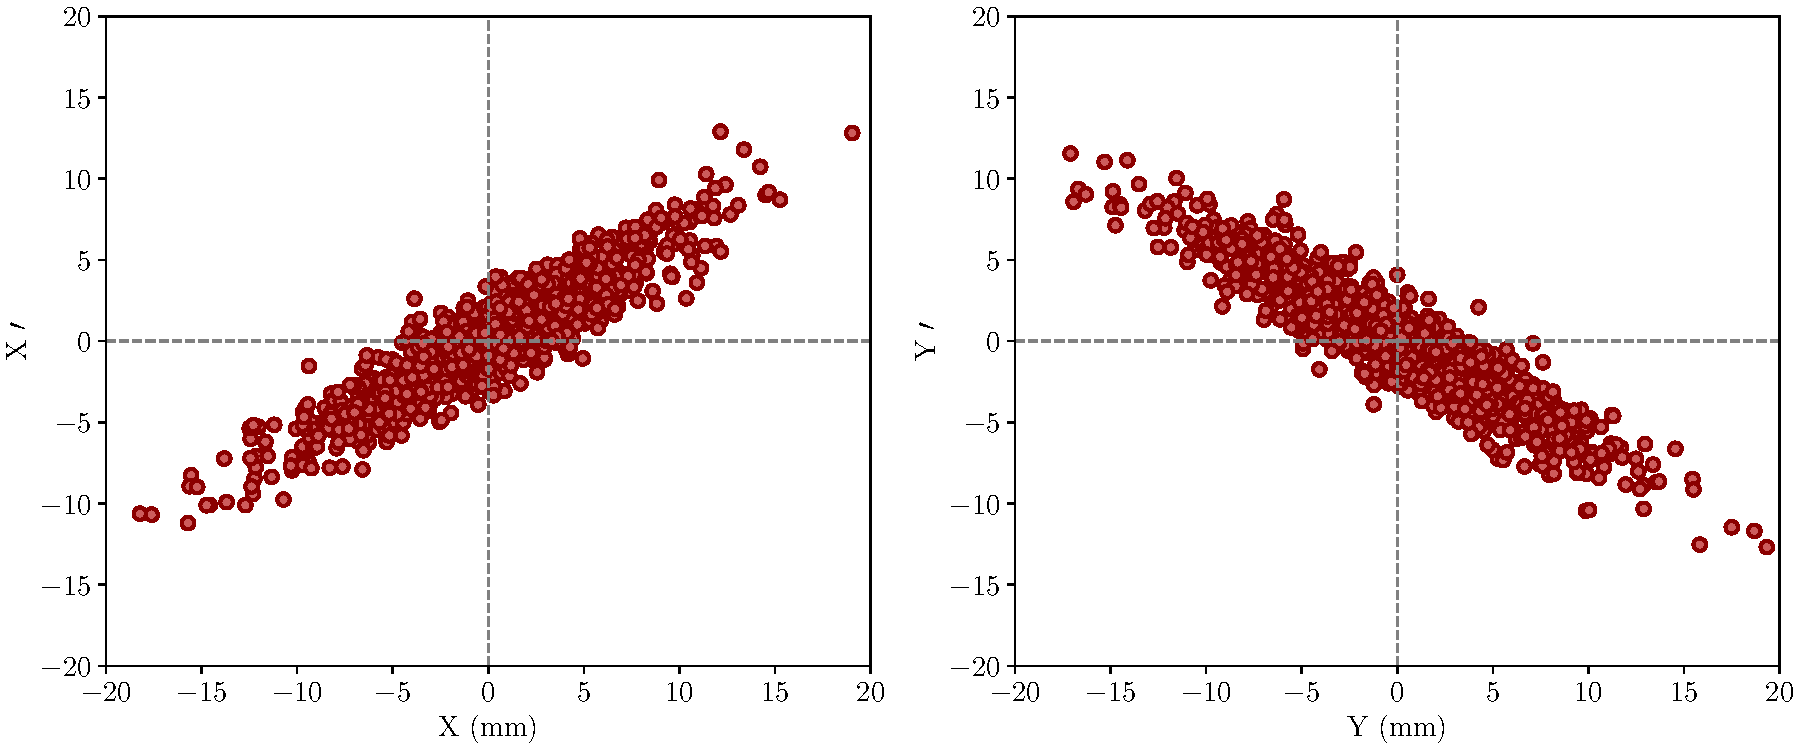
\includegraphics[width=1.0\columnwidth]{Figure_PhaseSpaceDist/PhaseSpaceDist.pdf}
    \caption{Particle distribution in the transverse phase space. }
    \label{fig:PhaseSpace}
\end{figure}

Because the velocity and the momentum of the particles are related, one can express the information of the phase space in terms of the transverse momenta of the particles $\left(p_x , p_y \right)$. For convenience, the phase space is described by the transverse momentum $(p_x , p_y)$ normalized by the longitudinal momentum $(p_s)$. This quantities are expressed by: $x^{'} = p_x / p_s$ and $y^{'} = p_y / p_s$. For representing the phase space, two charts are needed, one for the vertical plane and one for the horizontal plane.

Figure \ref{fig:PhaseSpace} shows an example of particle distribution in the phase space. From these figures, we can see that the distributions are ellipses, but in this case, they are tilted with respect to the axes. The phase space contains the whole description of the states of all the particles for a particular plane, and it is needed if to calculate the motion of the particles in the electromagnetic fields of the accelerator. 

\subsection{Transverse beam emittance}
\label{subsec:TransBeamEm}

A formal description of the phase space can be formulated by exploiting the elliptical shape of the phase space. The equation of the phase-space ellipse can be described as follows: 

\begin{equation}
    \epsilon = \gamma x^2 + 2\alpha x x^{'} + \beta x^{'2}
    \label{eq:ellipse}
\end{equation}

The parameters $\alpha, \beta, \gamma$ are referred to as the Courant-Synder parameters \parencite*[][]{ref:BookAccPhysics}. The area of the ellipse is simply $A = \pi \epsilon$. In the accelerator and beam physics language, the area in the phase space ($\epsilon$) containing the particles is called the emittance, statistical emittance, or more precisely it is called the rms-emittance. In the case of Gaussian beams, the concept of rms-emittance can be directly interpreted as the area containing a fraction (f) of ions. For example, it can be proven \parencite*[][]{ref:BookAccPhysics2},  that the curve of area $\epsilon$ should contain a $39\%$ of particles.

\begin{figure}[h]
    \centering
    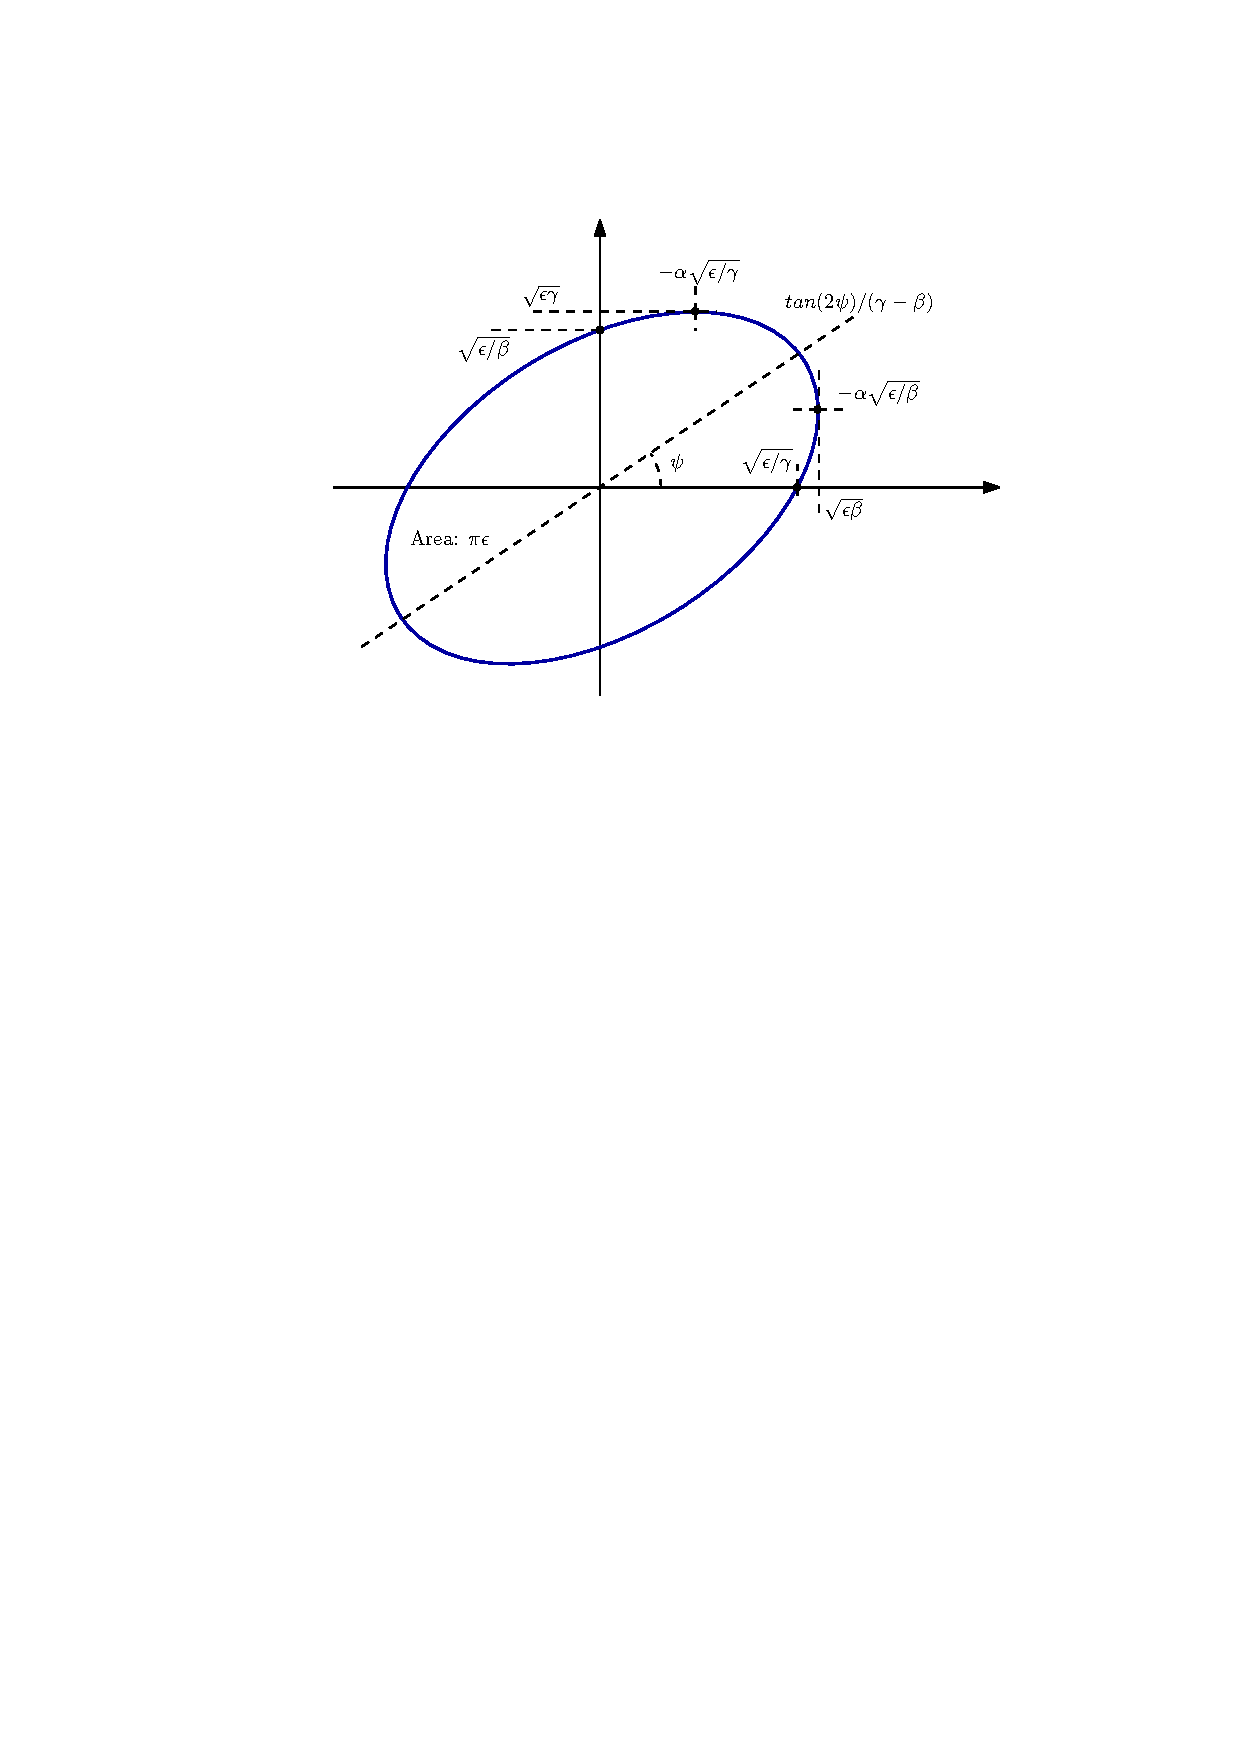
\includegraphics[width=0.7\columnwidth]{Figure_GeometricEmittance/GeometricEmittancve.pdf}
    \caption{Phase Space, geometrical ellipse. }
    \label{fig:CouranSnyder}
\end{figure}

    
Figure \ref{fig:CouranSnyder} shows a geometrical description of the Courant-Snyder parameters. These parameters $\left(\alpha, \beta, \gamma \right)$ are not independent, the third parameter is typically defined in terms of the other two: 

\begin{equation}
    \gamma = \frac{1 + \alpha^{2}}{\beta}
\end{equation}

Some other quantities, also very important for the understanding of the mathematical formulation of the transverse emittance are the following: 

\begin{equation}
    x_{rms}^2 = \left<x^2\right> =\frac{1}{N}\sum_{i=1}^N x_i^2
\end{equation}
\begin{equation}
    x_{rms}^{'2} = \left<x^{'2}\right> = \frac{1}{N}\sum_{i=1}^N x_i^{'2}
\end{equation}
\begin{equation}
    x x^{'}_{rms} =  \left< x x^{'}\right> = \frac{1}{N}\sum_{i = 1}^{N} x_{i} x^{'}_{i}
\end{equation}

With $x_{i} = X_{i} - \left< X \right>$ and $x^{'}_{i} = X_{i} - \left< X^{'}\right>$. $X_{i}$ and $X_{i}^{'}$ being the horizontal position and momentum of the individual particles conforming from the beam. For convenience these parameters can be expressed in a matrix form as follows: 

\begin{equation}
    \Sigma = 
    \begin{pmatrix}
        \left< x^{2} \right> & \left< x x^{'} \right> \\
        \left< x x^{'} \right> & \left< x^{' 2} \right>
    \end{pmatrix}
    = \epsilon 
    \begin{pmatrix}
        \beta & - \alpha \\ -\alpha  & \gamma
    \end{pmatrix}
\end{equation}

The rms-emittance ($\epsilon$) can also be obtained from these parameters: 

\begin{equation}
    \epsilon = \pi \sqrt{\left<x^{2}\right>\left< x^{'2}\right> - '\left<x x^{'}\right>^{2}}
\end{equation}



\subsection{Phase Space Evolution}
\label{subsec:PhaseSpaceEvol}

In a transfer line or a storage ring (i.e. no acceleration), and assuming no energy losses due to radiation, Liouville's theorem establishes that emittance ( considering both transverse and longitudinal coordinates) is conserved \parencite*[][]{ref:EmittanceConserv}.

\begin{figure}[h]
    \centering
    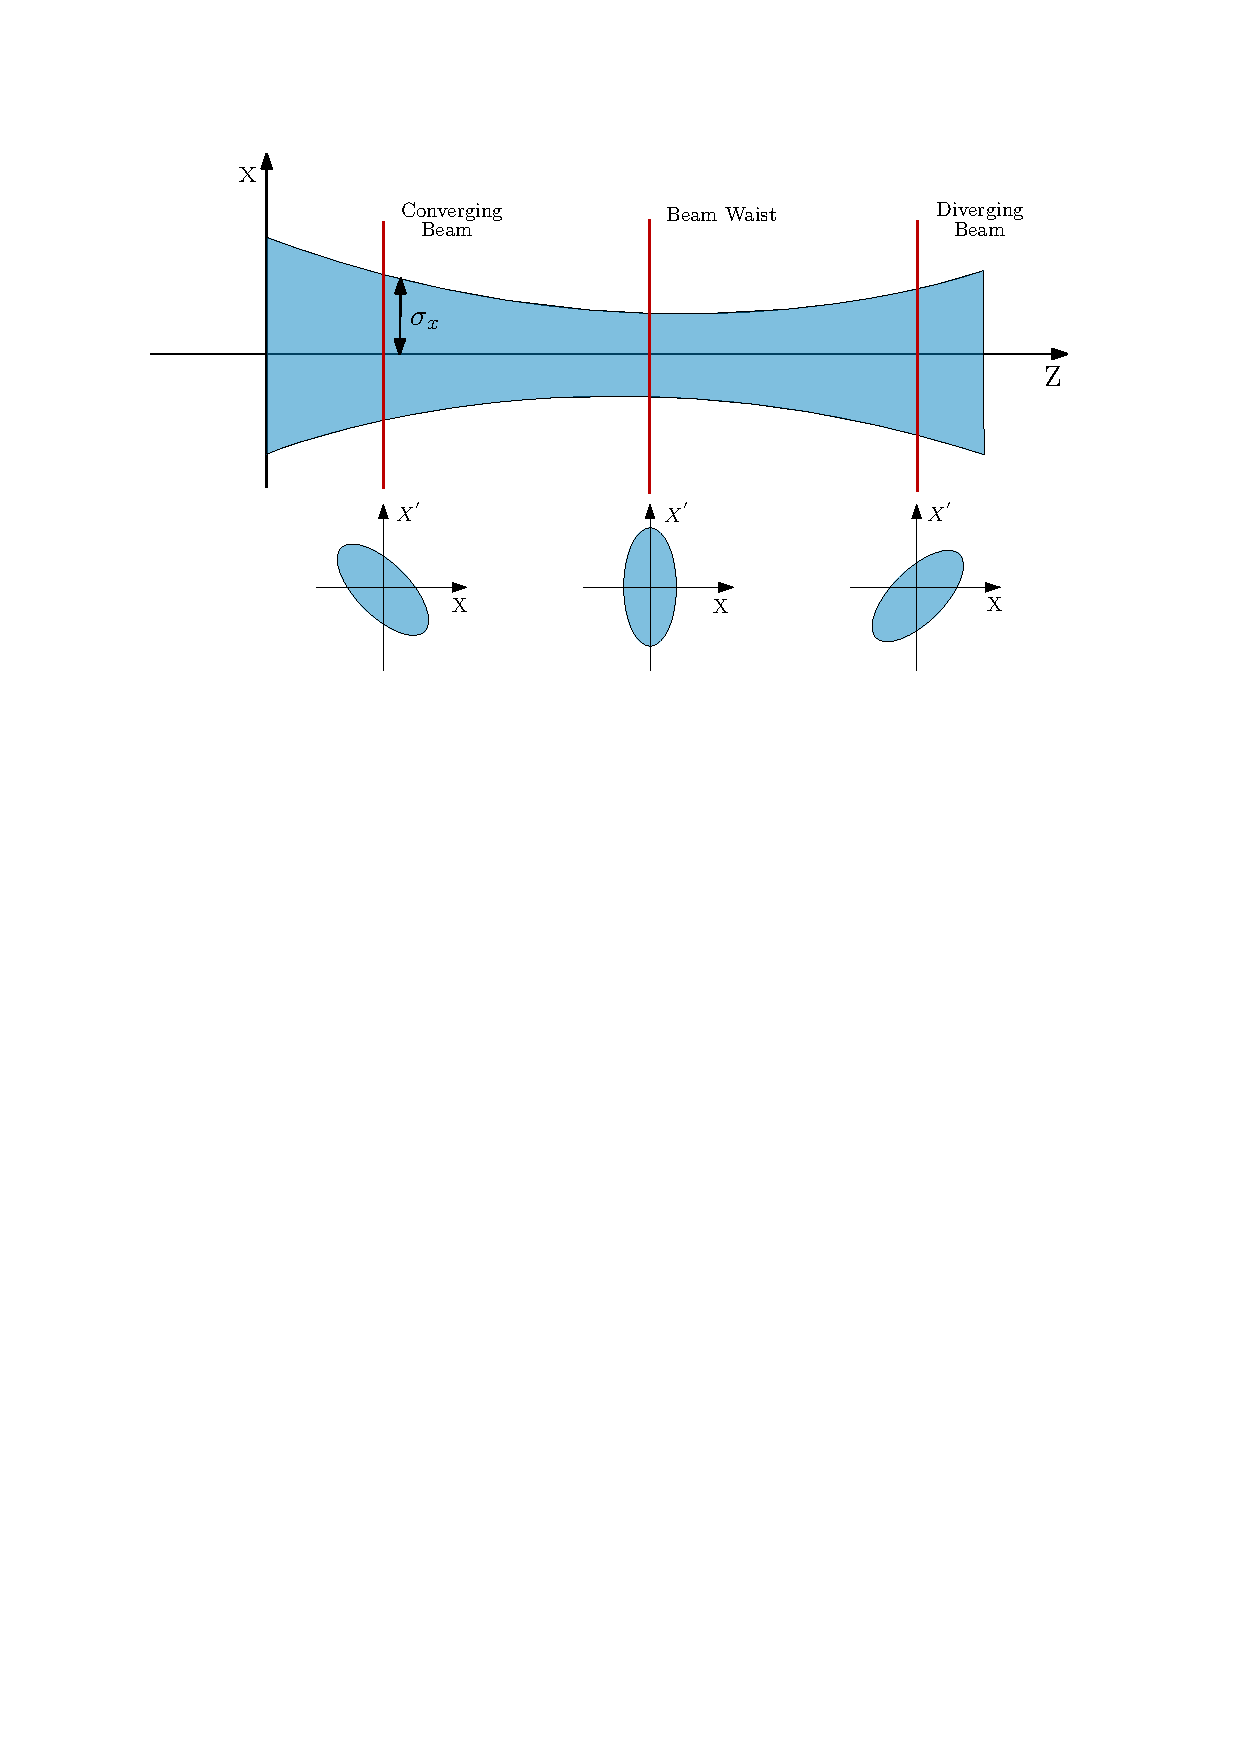
\includegraphics[width=0.85\columnwidth]{Figure_BeamEvolution/BeamEvolution.pdf}
    \caption{Example of phase space evolution. }
    \label{fig:PhasSpaceEvol}
\end{figure}

However, the shape of the ellipse changes along the beam line. Figure \ref{fig:PhasSpaceEvol} illustrates a typical example of phase space evolution. 
In the previous sections (Sec. \ref{subsec:PrincBeamDyn}) we saw how, in linear systems, points on the phase-space could be mapped from one location to the other through matrix multiplications. After some algebraic calculations, one can obtain the following transport matrix for the Twiss parameters \parencite*[][]{ref:MatrixToTwiss}:

\begin{equation}
    \begin{bmatrix}
       \beta_1 \\ \alpha_1 \\ \gamma_1
    \end{bmatrix}
    =
\begin{bmatrix}
   c^2 & - c s & s^2 \\ -c c^{'} & cs^{'} + c^{'}s & -s s^{'} \\ c^{'2} & -2c^{'}s^{'} & s^{'2}
\end{bmatrix}
=
\begin{bmatrix}
   \beta_0 \\ \alpha_0 \\ \gamma_0
\end{bmatrix}
\label{eq:MatrixEq}
\end{equation}

\section{Beam Diagnostics}

Beam diagnostics and instrumentation are essential constituents of any particle accelerator. They allow us to monitor the behavior and properties of the particle beam. Without adequate diagnostics, one would be blindly operating an accelerator and it would be impossible to assess problems and improve performances. Different accelerator types require different diagnostics. Similarly, different beam properties require very different instrumentation systems and techniques.  \parencite*[][]{ref:BeamInstrumentationBook}, \parencite*[][]{ref:NotesBeamInst} and \parencite*[][]{ref:CASbeamInst}, are very recommendable references, where the topic of beam instrumentation is covered extensively but yet with a very accessible approach. 

Here we will only focus on describing the instruments that are relevant for understanding this work. We shall focus on the measurements of two beam properties: 

\begin{itemize}
    \item Transverse Beam Profile Measurements: They allow the measurement of the transverse distribution of the particles throughout the accelerator. This measurement is important to control the beam width and position, as well as the transverse matching between different parts of the accelerator facility. In particular, we will focus on devices such as Secondary Emission Grids (SEM Grids) and Wire Scanners. 
    \item Beam Intensity Measurements: They allow us to measure the total electrical current of the beam. Current measurements allow, for example, to determine the transfer efficiencies in linacs and transfer lines. In this case, we will talk about Beam Current Transformers (BCT) and Faraday Cups (FC).
\end{itemize}

\subsection{Seconday Emission Grids (SEM Grids)}
\label{sec:SEMgrids}

Wire Grids or Secondary Electron EMission grids (SEM Grid) are devices composed of a large number of parallel fixed wires or strips. Figure \ref{fig:SEMgrid} shows an example of a SEM grid detector. They are interceptive devices, during the measurements, each one of the wires interacts directly with the beam of particles. During this process, a current, proportional to the number of particles, is generated in each wire.  By measuring the current in all the wires a beam profile can be reconstructed. More detailed explanations about the current generation process and the profile reconstruction will be given in Chapters \ref{ch:BeamMatterInter}.

\begin{figure}[h]
    \centering
    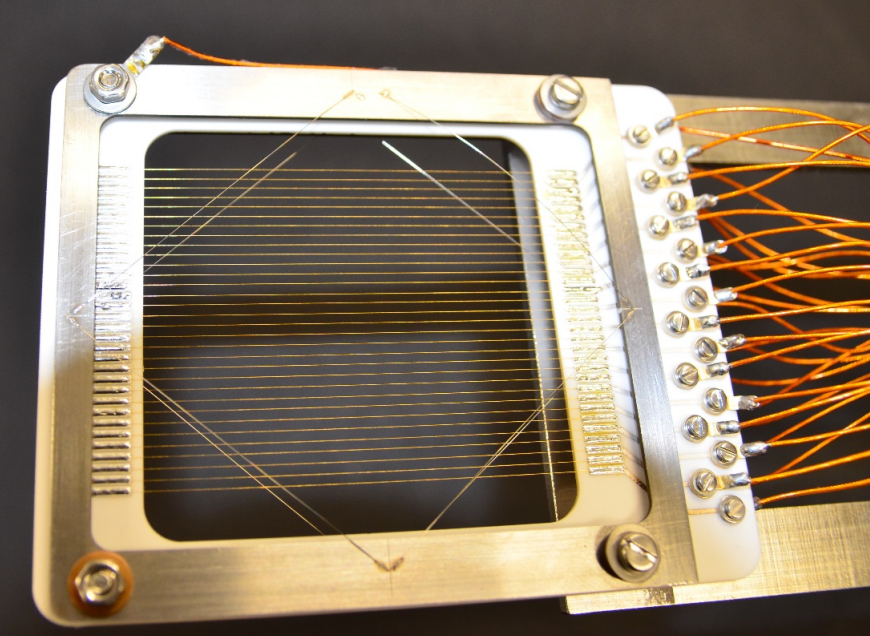
\includegraphics[width=0.6\columnwidth]{SEMGrid/semgrid.png}
    \caption{Example of a SEM grid installed at CERN accelerator Complex. }
    \label{fig:SEMgrid}
\end{figure}

SEM grids allow for a single-shot acquisition, and in some cases, it is possible to observe the evolution of the beam profile in the same pulse. The number of wires and the spacing between them varies from system to system. It is important for the detector to cover the whole range of the beam size and to have enough resolution to properly reconstruct the beam profile. Theoretically, a bigger detector with a larger number of wires would be more convenient. However, a system with too many wires implies an overly complicated acquisition system, it increases the probability of wire cross-talk and augments the construction costs. A typical number of wires ranges from 16 to 48. In some devices, the wires are spaced unevenly, with a denser distribution in the center. 

The diameter-to-spacing of the wires determines the attenuation of the beam current, which becomes an important parameter to consider for particles at low energies as they are fully stopped in the detector's material. It is common to consider that a $10 \%$ of the beam area is covered with wires. The wire materials are selected to optimize signal generation and ensure proper thermal performance. Typical materials used for wire grid designs are Tungsten, Carbon (Graphite, CNT) or Titanium. The motion control of SEM grids is relatively simple, they are either fully inserted or fully retracted, and sometimes they might even be permanently positioned in the beam pipe with no motion control at all. 

\begin{figure}[h]
    \centering
    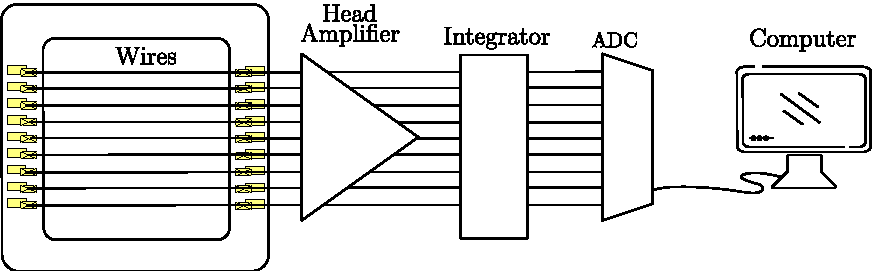
\includegraphics[width=0.9\columnwidth]{SEMgridDataADq/SEMdataAdc.pdf}
    \caption{Schematic representation of SEM Grid Acquisition system. }
    \label{fig:SEMGridReadOutSystem}
\end{figure}

Figure \ref{fig:SEMGridReadOutSystem} shows a schematic representation of the sem grid acquisition system. This system is composed of a head amplifier that sits as near as possible to the grid, often in an area with radiation. It is followed by an integrator or signal conditioning circuit that sits away in a safe room. From the integrator, the signal is fed to a computer controller ADC. This scheme requires one signal cable per wire over the distance from the device to the ADC \parencite[][]{ref:CASEnrico}. The main drawbacks of this diagnostics device are the limit on the spatial resolution (which can be hardly reduced to less than a few hundred micrometers), the small wire signals and the complicated data acquisition system. 

\subsection{Wire Scanners}
\label{sec:WireScan}

The Wire Scanners consist of a single wire that can be swept through the beam pipe (See figure \ref{fig:WireScan}). The main advantage of this technique is the high resolution that can be accomplished (sub-mm range). It is often used in accelerators with small beam sizes. These devices also intercept the beam of particles, however, its effect is practically negligible. The electronics and read-out system is simpler than the SEM grids. However, the mechanical design of the mechanism is much more challenging.

\begin{figure}[h]
    \centering
    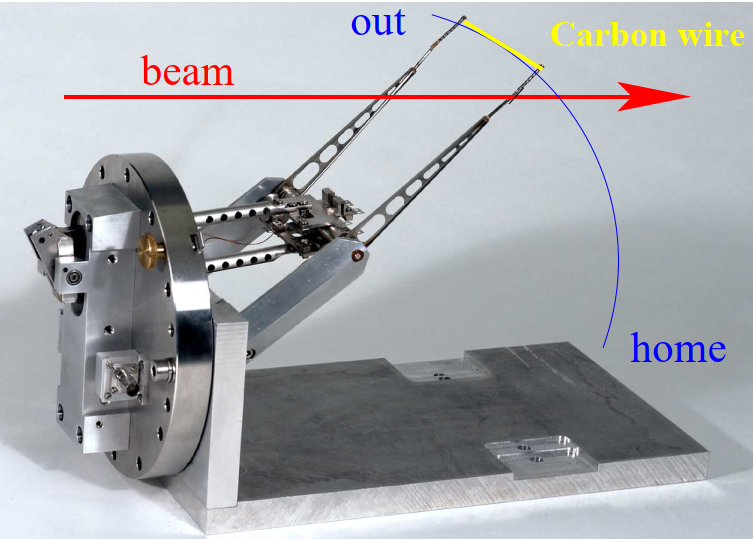
\includegraphics[width=0.6\columnwidth]{WireScanner/WireScanner.png}
    \caption{Rotational Fast Wire Scanner, used at CERN SPS. }
    \label{fig:WireScan}
\end{figure}

In the context of this thesis, we differentiate between two types of wire scanners:

\begin{enumerate}
    \item Slow Wire Scanners: They are commonly used on LINACs or transfer lines. Where the beam energy of the particle beam is small and the pulse structure consists of short pulses and low repetition rates. In this case, the profile is reconstructed by using the current generated in the detector by its interaction with the beam of particles. Due to the low repetition rate of the beam in those areas, one sample is taken on each beam pulse.
    \item Fast Wire Scanners: For high energy and high repetition range beams, the profile is reconstructed by measuring a shower of secondary particles generated during the beam/wire interaction (for proton/heavy ion accelerators).  The secondary shower is detected outside the beam pipe, with a photo-multiplier tube. The speed of the wire movement varies can go from 1 \si[]{\metre /\second} up to 20 \si[]{\meter /\second}. 
\end{enumerate}

In both cases, the measurement of the wire position is a crucial aspect of the measurement, as the beam profile is reconstructed by correlating the wire position with the generated signal. The precision of the measurements of the wire scanner positions will therefore be a crucial factor in the measurement precision and resolution. In the case of fast wire scanners, the deformations or vibrations in the wire can also restrict spatial resolution. Beam position and beam size variations during the measurement period can induce additional errors. 

For both, slow and fast wire scanners, the dimensions of the wire have a direct impact on the signal strengths and the measurement accuracy. In general wire sizes between 10 \si[]{\micro \metre} to 50 \si[]{\micro \metre}  are used.

\section{Beam Current Transformer (BCT)}
\label{sec:BCT}

An electric current flowing through a conductor gives rise to a magnetic field around the conductor, and passing a conducting loop through a magnetic field induces a current through the loop. These well-known principles of induction are used in the Beam Current Transformer (BCT). In this case, the particle beam is the primary current and can be described as: 

\begin{equation}
    I_{beam} = \frac{q e N_{part}}{t}
\end{equation}

Where $N_{part}$ is the number of particles of charge $q$ per unit time $t$. $e$ is the electron charge. A magnetic field is generated as the beam travels through the accelerator. One can measure this magnetic field by placing torus with high permeability around the beam. Some windings are placed around the torus and then connected to an electrical circuit for read-out. Figure \ref{fig:BCTschema} shows a schematic representation of a BCT design. Measuring small beam currents becomes very challenging with these devices.

\begin{figure}[h]
    \centering
    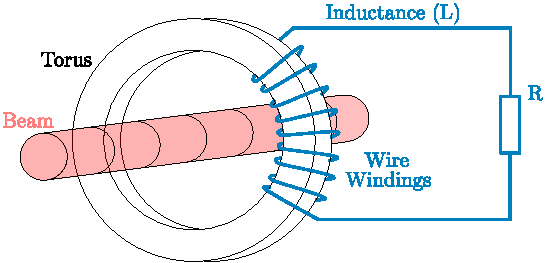
\includegraphics[width=0.6\columnwidth]{BCTschema/BCTschema.pdf}
    \caption{Schema of a current transformer built as a ring-core (torus). }
    \label{fig:BCTschema}
\end{figure}

\section{Faraday Cup (FC)}
\label{sec:FC}

A faraday cup (FC) is a beam stopper that measures the electrical current of the beam. A basic cup design is shown in figure \ref{fig:FaradayCup}. With a Faraday cup, a much lower current can be measured compared to a BCT, of the order of the \si[]{\pico \ampere} for low noise systems. These devices consist of an isolated metal cup connected to a current-sensitive pre amplifier. The current in these detectors is generated by measuring the total charge from the beam of particles that are deposited in them. High energetic particles not depositing all their energy in the detector material can affect negatively the measurement results. Similarly, a Secondary Electron (SE) suppression system has to be included in these devices to avoid errors in the current measurements. This is done by creating very long cups, putting high voltage suppression close to the entrance or by using a magnetic field. 

Sometimes, Faraday cups are also used for higher beam currents, where measurements with BCTs are also possible as they are easier to implement. In addition, cups serve as beam dumps. For high beam energies, one has to be concerned about the high thermal and structural shocks that these devices might suffer.

\begin{figure}[h]
    \centering
    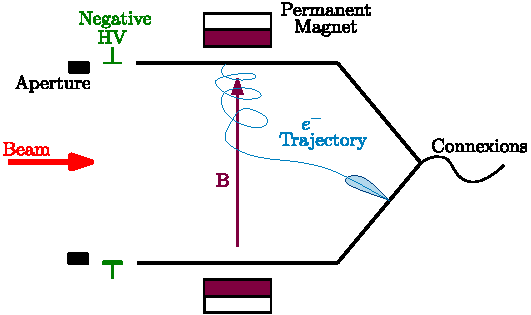
\includegraphics[width=0.6\columnwidth]{FCschema/FCschema.pdf}
    \caption{Schematic Representation of Faraday Cup. }
    \label{fig:FaradayCup}
\end{figure}
